\documentclass[]{article}
\usepackage[]{graphicx}
\title{Power Outage Poller: Purpose and Progress}
\author{Jacob Pavelka}

\begin{document}
\maketitle

The purpose of this project is to gather all information available from our communicating devices and external sources to better inform decision-making processes.

Currently, this project's main focus is gathering power outage data to combat severe weather events. To do this, we use Selenium's Webdriver to scrape information about electricity meter status from Oncor's website. We then use that to determine whether communication failures between our management facility and the traffic signal are caused by a lack of power. This helps us diagnose issues with our traffic signals. However, in our projects current state, the information is gathered from the web but remains in an offline database. We wish to integrate this data with our current GIS data, displaying power outage information on MAXVIEW through ArcGIS Online (AGO) and enhancing our response to weather events.

We require your aid in setting up a mechanism to transfer our separately generated database to AGO on a regular basis, then have AGO synchronize with MAXVIEW, our Advanced Traffic Management system.

The rest of this document contains details on the current state of our project. As mentioned before, we are using Selenium's Webdriver to scrape power outage data from Oncor's website. This process begins with a list of known "ESI ID", which uniquely mark each power meter that is servicing the city's traffic signals. A typical list of ESI ID's are shown in Figure~\ref{fig:ids}.
\begin{figure}[htbp]
    \centering
    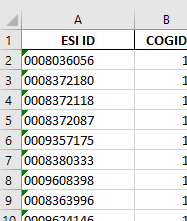
\includegraphics{esi_id.PNG}
    \caption[short]{An example list of ESI IDs}
    \label{fig:ids}
\end{figure}
The Webdriver takes each id from this list, inserts it into the Oncor's web GUI, and then requests information about the meter's status. Interaction with Oncor's webpage is shown in Figure~\ref{fig:oncor_in}. 
\begin{figure}[h]
    \centering
    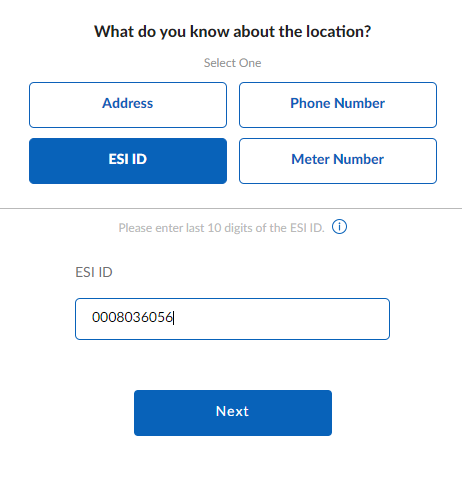
\includegraphics[width=0.6\textwidth]{oncor_esi_in.PNG}
    \caption{GUI interface in which ESI ID's are inputted}
    \label{fig:oncor_in}    
\end{figure}
A new webpage loads based on this process, and it is parsed to update the meters status. A typical webpage that is loaded is shown in Figure~\ref{fig:oncor_out}.
\begin{figure}[h]
    \centering
    
\includegraphics[width=0.6\textwidth]{oncor_status.PNG}
    \caption{Results generated from Oncor's GUI}
    \label{fig:oncor_out}    
\end{figure}
Scraping Oncor's web GUI like this is a lengthy process currently, taking over an hour to update all meters, but we hope to improve this speed later on. In any case, this process can be ran continuously, providing a full update every hour. Currently, the results are stored on a local database. The next task is to upload the results hourly to our interfaces.

\end{document}